What is Power Electronics?

\begin{define}
\textbf{Source:} something that generates power

\textbf{Load:} something that consumes power

\textbf{Power electronics:} application of electronics and circuitry to control the conversion of one form to another
\end{define}

Converter types between AC and DC Power: DC stands for "direct current" and can be visualized as a constant voltage over time. One example is a battery and photovoltaic panel. AC power stands for "alternating current" and is a sinusoidal voltage in time. An example of this is the power from the outlet. There are four basic types of converters.
\begin{itemize}
    \item AC-DC: AC source to DC load, which is commonly called a rectifier like in the use of a laptop charger
    \item DC-DC: DC source to DC load, battery pack USB
    \item DC-AC: DC source to AC load, also commonly called an inverter like for a photovoltaic to grid system
    \item AC-AC: AC source to AC load, not as common but used in wond power system
\end{itemize}

\subsection{Average and Root Mean Square (RMS) Calculations}
Period waveforms repeat their shape across each period. The average value of a sine wave is 0. $\langle v(t) \rangle = \frac{1}{T} \int_0^T v(t) \,dt$ will represent the average value here.

The RMS is represented as capital V listed below
\begin{define}
    \[V = \sqrt{\frac{1}{T} \int_0^T v(t)^2 \,dt}\]
\end{define}
We can think of the RMS value as the equivalent voltage if we put the waveform of choice across a resistor

The power is equal to the voltage waveform squared over the resistor. The triangle brackets represent the average here.
\begin{define}
    \[\langle P \rangle = \langle \frac{v^2}{R} \rangle = v^2\]
\end{define}
Remember that 
\[\langle v \rangle ^2 \neq v^2\]

If we take a look at this sine wave and say that this represents current and connected this to a resistor, average power would not be 0 even though average current is 0. $I(t)$ here represents the instantaneous value. The resistor generates (consumes) power at both the negative and positive parts of this waveform.
\begin{center}
    \begin{tikzpicture}
        % Axes
        \draw[->] (0,0) -- (6.5,0) node[right] {$t$};
        \draw[->] (0,-1.5) -- (0,1.5) node[above] {$I(t)$};
        
        % Sine wave
        \draw[domain=0:2*pi,smooth,variable=\x,blue] plot ({\x},{sin(\x r)});
        
        % Labeling
        \draw[dashed] (pi/2,0) -- (pi/2,1) node[pos=0.5, right] {$\frac{\pi}{2}$};
        \draw[dashed] (3*pi/2,0) -- (3*pi/2,-1) node[pos=0.5, left] {$\frac{3\pi}{2}$};
        
        % Axes labels
        \node[below] at (pi,0) {$\pi$};
        \node[below] at (2*pi,0) {$2\pi$};
        \node[left] at (0,1) {1};
        \node[left] at (0,-1) {-1};
    \end{tikzpicture}
\end{center}

\begin{sanity}
    Is the RMS value always greater than or equal to the average value? Yes. Recall the definitions of average value and the RMS value above. My intuition behind this is that you're squaring a periodic function there will be no negative values.
\end{sanity}

Sine wave RMS value calculations:

Define $x(t) = X_{peak} \sin{(t \times \frac{2\pi}{T})}$. We multiply $t$ by a factor of $\frac{2\pi}{T}$ since we are working in units of time.
\begin{align*} 
    X_{RMS} &= \sqrt{\frac{1}{T} \int_0^T X_{peak}^2 \sin^2{(t \times \frac{2\pi}{T})} \,dt} \tag{1} \\
    &= \sqrt{\frac{X_{peak}^2}{T} \int_0^T (1-\cos{(2\cdot \frac{2\pi}{T})}) \,dt} \tag{2} \\
    &= \sqrt{\frac{X_{peak}^2}{2T} \left[t \mid_0^T - \sin{(\frac{4\pi t}{T})\frac{T}{4\pi} \mid_0^T}\right]_0^T} \tag{3} \\ 
    &= \sqrt{\frac{X_{peak}^2}{2T} \left[T - \frac{T}{4\pi}(\sin{(4\pi) - \sin{(0))}}\right]_0^T} \tag{4} \\
    &= \frac{X_{peak}}{\sqrt{2}} \tag{5}
\end{align*}

Line (2) comes from the trig idenity 
\[\sin^2{u} = \frac{1-\cos{(2u)}}{2}\]
Line (3) comes from evaluating the integral. In line (4), we see that everything within the brackets evaluates to $T$ and that this results in $T$ cancelling out with the $T$ in the denominator, resulting in just a 2 in the denominator, which is later square rooted.

\subsubsection{$X_{peak}$ and Oscilloscope Readings}
We notice that $X_{peak}$ is described in its RMS value as the large value that we can get. The amplitude of this sine wave is 1, but if we were to output this sinusoid in High-Z mode on the function generator, we would have to set this to a 2 $V_{pp}$ (Volt peak to peak). Contrastingly, if we were in 50-Ohm mode, setting the function generator to 2 $V_{pp}$ would result in a sinusoid with an $X_{peak}$ of 4 $V$.

Why is my function generator's output voltage wrong?
\begin{enumerate}
    \item \textbf{Scope vertical scale is using wrong probe attenuation.} A lot of scopes set this vertical scale automatically for you, so you may have to set this scale to be larger or smaller depending on how large your voltage is.
    \item \textbf{Load impedance is different from what the generator expects.} Image a voltage divider below. If our function generator wants to output 1 $V_{pp}$ at $R_{load}$ then, if $R_f = 50 \Omega$ and it assumes the $R_{load}$ is also $50 \Omega$ then that means thats the function generation will set $V_s$ as $2 V_{pp}$. However, sometimes it is the case that if $R_{load}$ is too high (such as in the case of the oscilloscope itself) then that means that voltage drop across $R_f$ is not that big and most of the voltage drop occurs across $R_f$. This results in us reading 2 $V_{pp}$ when we meant to output 1 $V_{pp}$. To correct this, correct the load impedance on the function generator settings if you have the setting for it to High-Z or what your load impedance on whatever you're connecting to is or connect a 50 $\Omega$ through terminator to your coax on your lead.
    \begin{center}
        \begin{circuitikz}[american]
            \draw (0,0) to[sinusoidal voltage source, v=$V_{\text{s}}$] (0,-2);
            \draw (0,0) to[R, l=$R_{f}$, v=$V_1$] (3,0);
            \draw (3,0) to[R, l=$R_{load}$, v=$V_2$] (3,-2);
            \draw (0,-2) -- (3,-2);
            \draw (3,0) -- (4,0) node[right] {$V_{\text{out}}$};
        \end{circuitikz}
    \end{center}
\end{enumerate}

\subsection{Real, Reactive and Apparent Power}
There are three different types of AC power. $\phi$ here is the impedance phase angle between the voltage and the current.
\begin{define}
    \textbf{Apparent power:} product of the RMS current and RMS voltage and represented by S in units of VA
    \[S = V_{RMS} I_{RMS}\]
    \textbf{Active/Real power:} power consumed or used within an AC circuit and represented by P. Is the real power in units of W (watts)
    \[P = V_{RMS} I_{RMS} \cos{\phi}\]
    \textbf{Reactive power:} the power developed in the circuit and represented by Q in units of VAR. Is the maximum value of the power component that "messes around", going back and forth
    \[Q = V_{RMS} I_{RMS} \sin{\phi}\]
\end{define}

We can describe the differences between apparent, reactive, and real power with a "sending a package analogy". The item you want to ship is your real power. To deliver power, you need a container, which is your apparent power. This has the potential to send an amount of power. However, you need some packaging in the container to cushion your item, which is your reactive power.
\begin{itemize}
    \item Real - item. Reactive loads like inductors and capacitors dissipate zero power
    \item Reactive - packaging. The actual amount of power being used or dissipated
    \item Apparent - box. This is the combination of reactive and real power and is without reference to phase angle.
\end{itemize}

\subsubsection{Pure Load Examples}


\begin{center}
    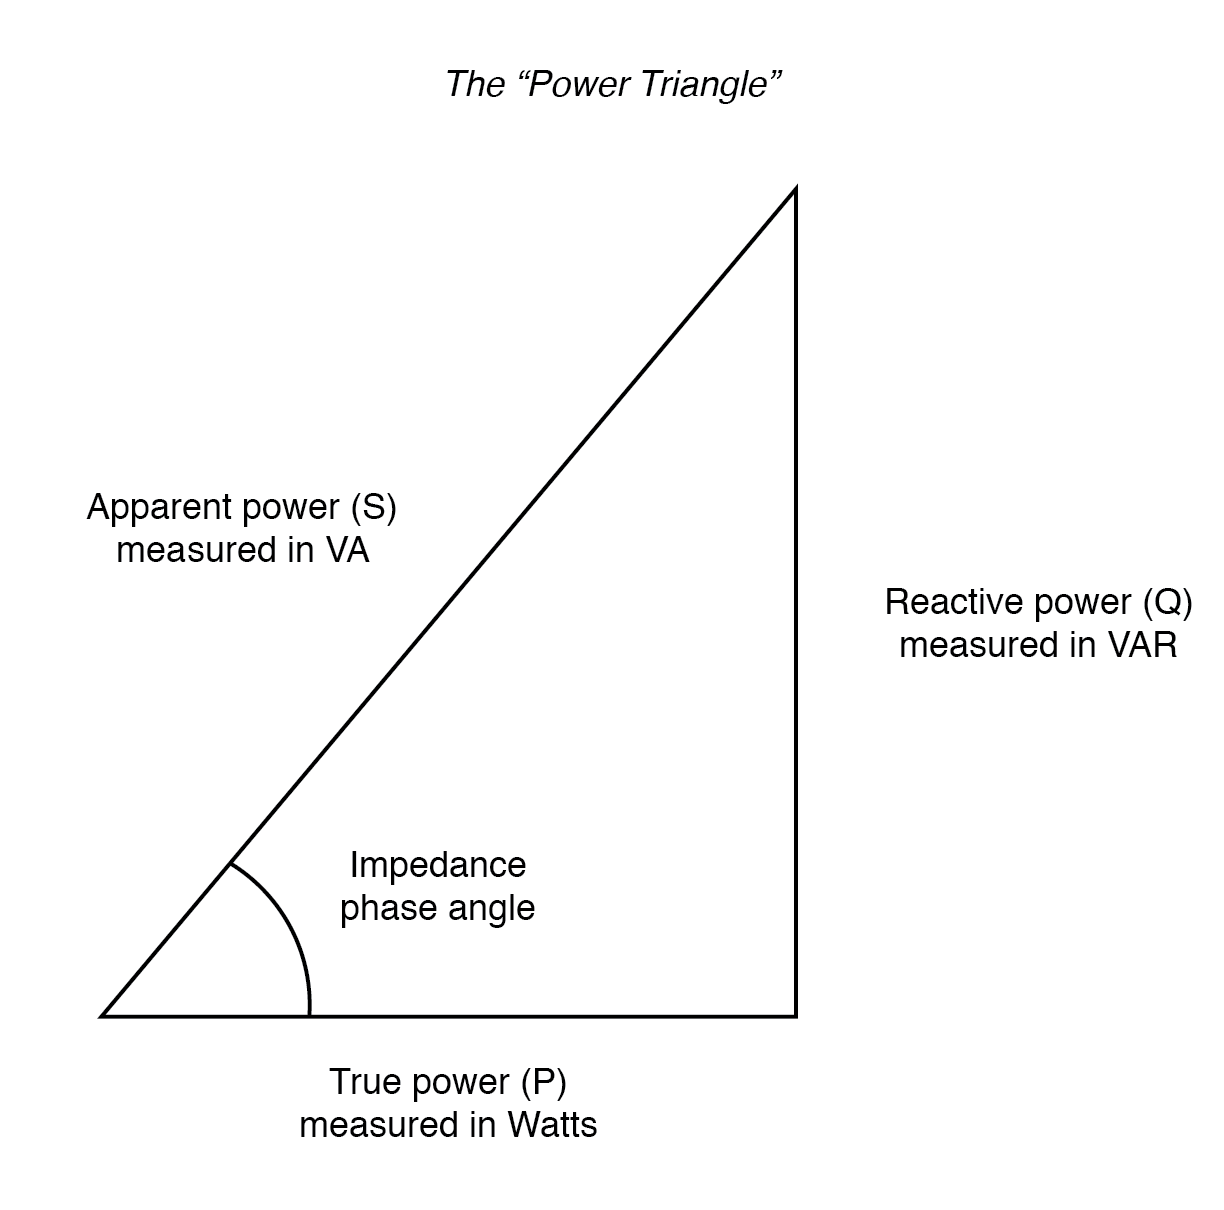
\includegraphics[scale=0.2]{figs/1_1_2_power_triangle.png}
\end{center}